  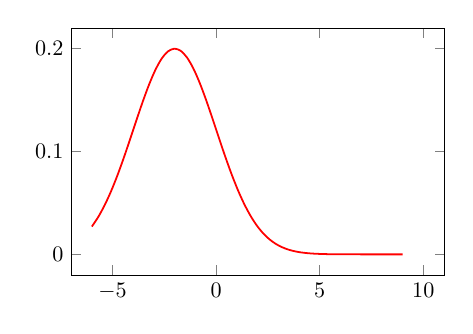
\begin{tikzpicture}[
    declare function={
      normalpdf(\x,\mu,\sigma)=
      (2*3.1415*\sigma^2)^(-0.5)*exp(-(\x-\mu)^2/(2*\sigma^2));
    },
    hplot/.style={ycomb, mark=o, dashed}, ,scale=0.8]
  
    \begin{axis}[
      width=7.5cm, height=5.5cm,
      samples=50,
      legend style={draw=none, fill=none},
      domain=-6:9,
      legend cell align=left,
      xmin=-7, xmax=11]
  
      \addplot [smooth, thick, red] {normalpdf(x,-2,2)} node[] {};
    \end{axis}
  \end{tikzpicture}
  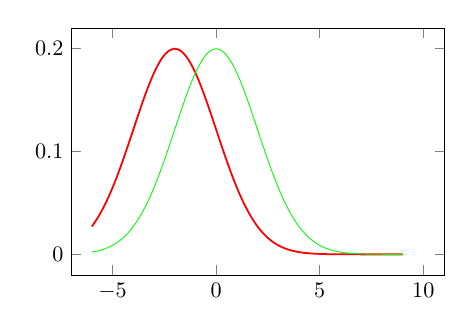
\begin{tikzpicture}[
    declare function={
      normalpdf(\x,\mu,\sigma)=
      (2*3.1415*\sigma^2)^(-0.5)*exp(-(\x-\mu)^2/(2*\sigma^2));
    },
    hplot/.style={ycomb, mark=o, dashed}, ,scale=0.8]
  
    \begin{axis}[
      width=7.5cm, height=5.5cm,
      samples=50,
      legend style={draw=none, fill=none},
      domain=-6:9,
      legend cell align=left,
      xmin=-7, xmax=11]
  
      \addplot [smooth, thick, red] {normalpdf(x,-2,2)} node[] {};
      \addplot [smooth, green] {normalpdf(x,0,2)} node[] {};
    \end{axis}
  \end{tikzpicture}

\begin{columns}

  \begin{column}{0.5\textwidth}

    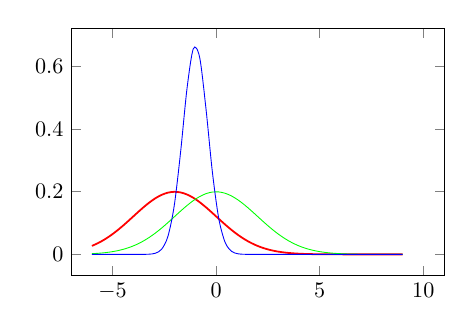
\begin{tikzpicture}[
      declare function={
        normalpdf(\x,\mu,\sigma)=
        (2*3.1415*\sigma^2)^(-0.5)*exp(-(\x-\mu)^2/(2*\sigma^2));
      },
      hplot/.style={ycomb, mark=o, dashed}, ,scale=0.8]
    
      \begin{axis}[
        width=7.5cm, height=5.5cm,
        samples=50,
        legend style={draw=none, fill=none},
        domain=-6:9,
        legend cell align=left,
        xmin=-7, xmax=11]
    
        \addplot [smooth, thick, red] {normalpdf(x,-2,2)} node[] {};
        \addplot [smooth, green] {normalpdf(x,0,2)} node[] {};
        \addplot [smooth, blue] {normalpdf(x,-1,0.6)} node[] {};
      \end{axis}
    \end{tikzpicture}
  \end{column}

  \begin{column}{0.5\textwidth}
    \begin{block}{}
      \begin{equation*}
        bel(x_t) = \eta p(z_t| x_t) \int p(x_t| u_t, x_{t-1}) bel(x_{t-1})dx_{t-1}
    \end{equation*}
    \end{block}
  \end{column}
\end{columns}